\section{Planning}%
\label{sec:orga82318d}
In fig.~\ref{fig:gantt-diag-orig} is illustrated the Gantt chart for the project, containing the tasks' descriptions. It should be noted
that the project tasks of Analysis, Design, Implementation and Tests are
performed in two distinct iterations as corresponding to the Waterfall project
methodology.

Due to unpredictable circumstances, limiting the mobility of team
staff and goods, the implementation stage will not be done at full extent, but
rather at a simulation stage. Thus, to overcome these constraints, the project
focus is shifted to the simulation stage, where an extensive framework as to
built to model the system operation, test it, and providing valuable feedback
for the dependents modules. As an example, the modules previously connected just
by an RS232 link, must now include upstream a web module (TCP/IP) --- the data
is now effectively sent through the internet, and must be unpacked and delivery
serially as expected if only the RS232 link was used.

The tasks are described as follows:
\begin{itemize}
\item \uline{Project Kick-off}: in the project kick-off, the group is formed and the tutor
is chosen. A brainstorming about conceivable devices takes place, whose
viability is then assessed, resulting in the product concept definition
(Milestone 0).
\item \uline{State of the Art}: in this stage, the working principle of the device is
studied based on similar products and the system components and its
characteristics are identified.
\item \uline{Analysis}: In the first stage --- Analysis 1 --- contains the analysis
results of the state of the art. It should yield the specifications document,
containing the requisites and restrictions to the project/product, on a
quantifiable basis as required to initiate the design; for example, the
vehicle's desired speed should be, at maximum, \texttt{2 m/s}. The second stage --- Analysis 2
--- contains the analysis of the first iteration of the development cycle.
\item \uline{Design}: it is done in two segments: modules design --- where the modules are
designed; integration design --- where the interconnections between modules is
designed. It can be subdivided into \emph{conceptual design} and \emph{solution
design}. 
\begin{itemize}
\item In the conceptual design, several problem solutions are identified,
quantifying its relevance for the project through a measuring scale,
inserted into an evaluation matrix, for example, QFD.%
\item In the solution design, the selected solution is developed. It must include
the solution modelling, e.g.:
\begin{itemize}
\item \uline{Control system}: analytically and using simulation;
\item \underline{Transducer design}: circuit design and simulation;
\item \uline{Power system}: power supply, motors actuation and
  respective circuitry design and simulation;
\item \uline{Communications middleware}: communication protocols evaluation and
  selection;
\item \uline{Software layers}: for all required modules, and considering its
  interconnections, at distinct levels:
  \begin{itemize}
  \item \uline{front end layer}: user interface software, providing a easy and convenient
    way for the user to control and manage the system.
  \item \uline{framework layer}: software required to emulate/simulate and test the
    required system behaviour, providing seamless interfaces for the dependents
    modules
  \item \uline{back end layer}: software running \emph{behind the scenes}, handling user
    commands received, system monitoring and control.
  \end{itemize}
\end{itemize}
\end{itemize}
\item \uline{Implementation}: product implementation which is done by
  \uline{modular integration}. In the first stage, the implementation is done in a prototyping
environment --- the assisting framework developed, yielding version alpha; in the second stage
it must include the coding on the final target modules, yielding
prototype beta.
\item \uline{Tests}: modular tests and integrated tests are performed. Tests are generally considered as those performed over any physical
component or prototype. Here, it is used as a broader term, to reflect the tests
conducted into the system and the several prototypes.
\item \uline{Functional Verification/Validation}: System verification may be performed to validate overall
  function, but not for quantifiable measurement, due to the latencies
  involved. Regarding validation, specially for an external agent, thus, it should be limited
  to user interface validation.
\item \uline{Delivery}: --- project closure encompassing:
\begin{enumerate}
\item Final prototype
\item Support documentation: how to replicate, instruction manual.
\item Final report
\item Public presentation
\end{enumerate}
\end{itemize}
%
%%%%%%%%%%%%%%% Figure is deprecated: use PDF instead
%\begin{figure}[!htbp]
%\centering
%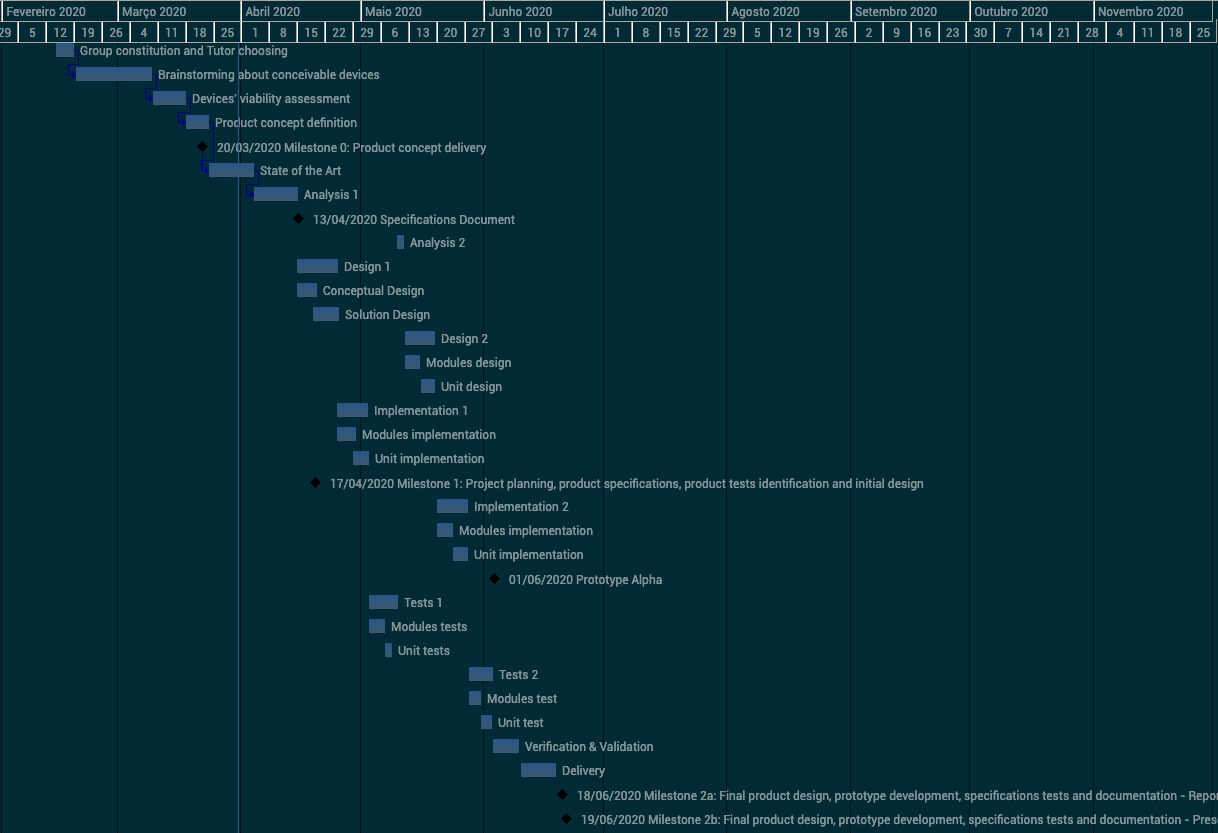
\includegraphics[width=1.0\textwidth]{./sec/img/gantt-diag-orig.png}
%\caption{\label{fig:gantt-diag2}Project planning: Gantt diagram 1}
%\end{figure}
%\begin{figure}[!htbp]
%\centering
%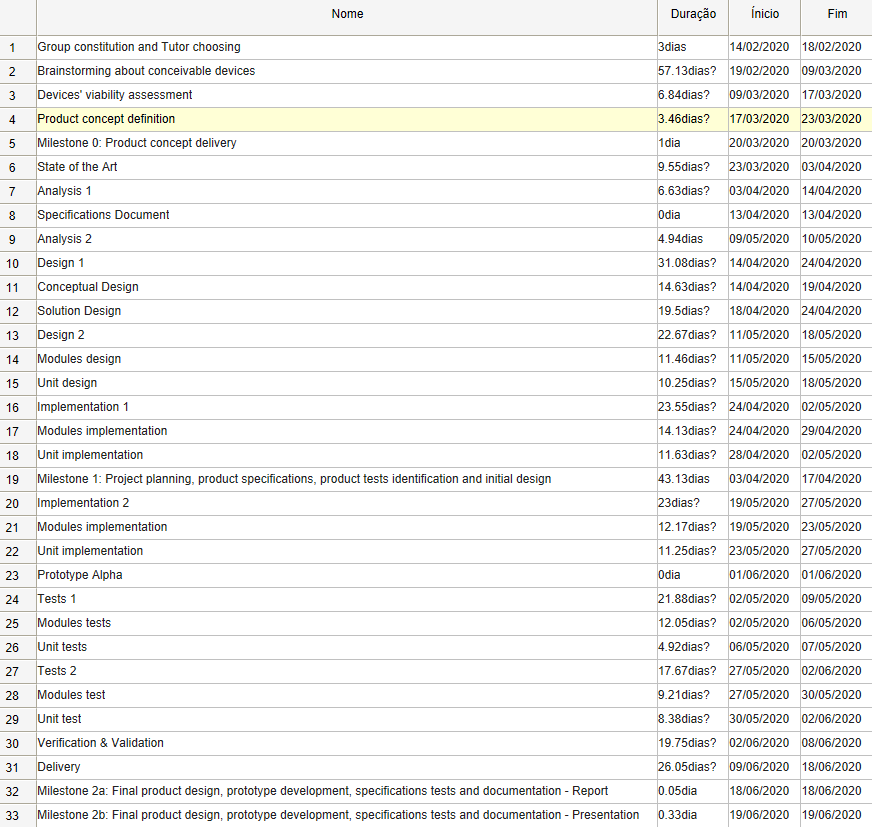
\includegraphics[width=1.0\textwidth]{./sec/img/gantt-orig-tasks.png}
%\caption{\label{fig:gantt-tasks}Project planning: tasks}
% \end{figure}
%%%%%%%%%%%%%%%%%%%%%%%%%%%%%%%%%%%%%%%%%%%%%%%%%%%%%%%%%%%%%
% 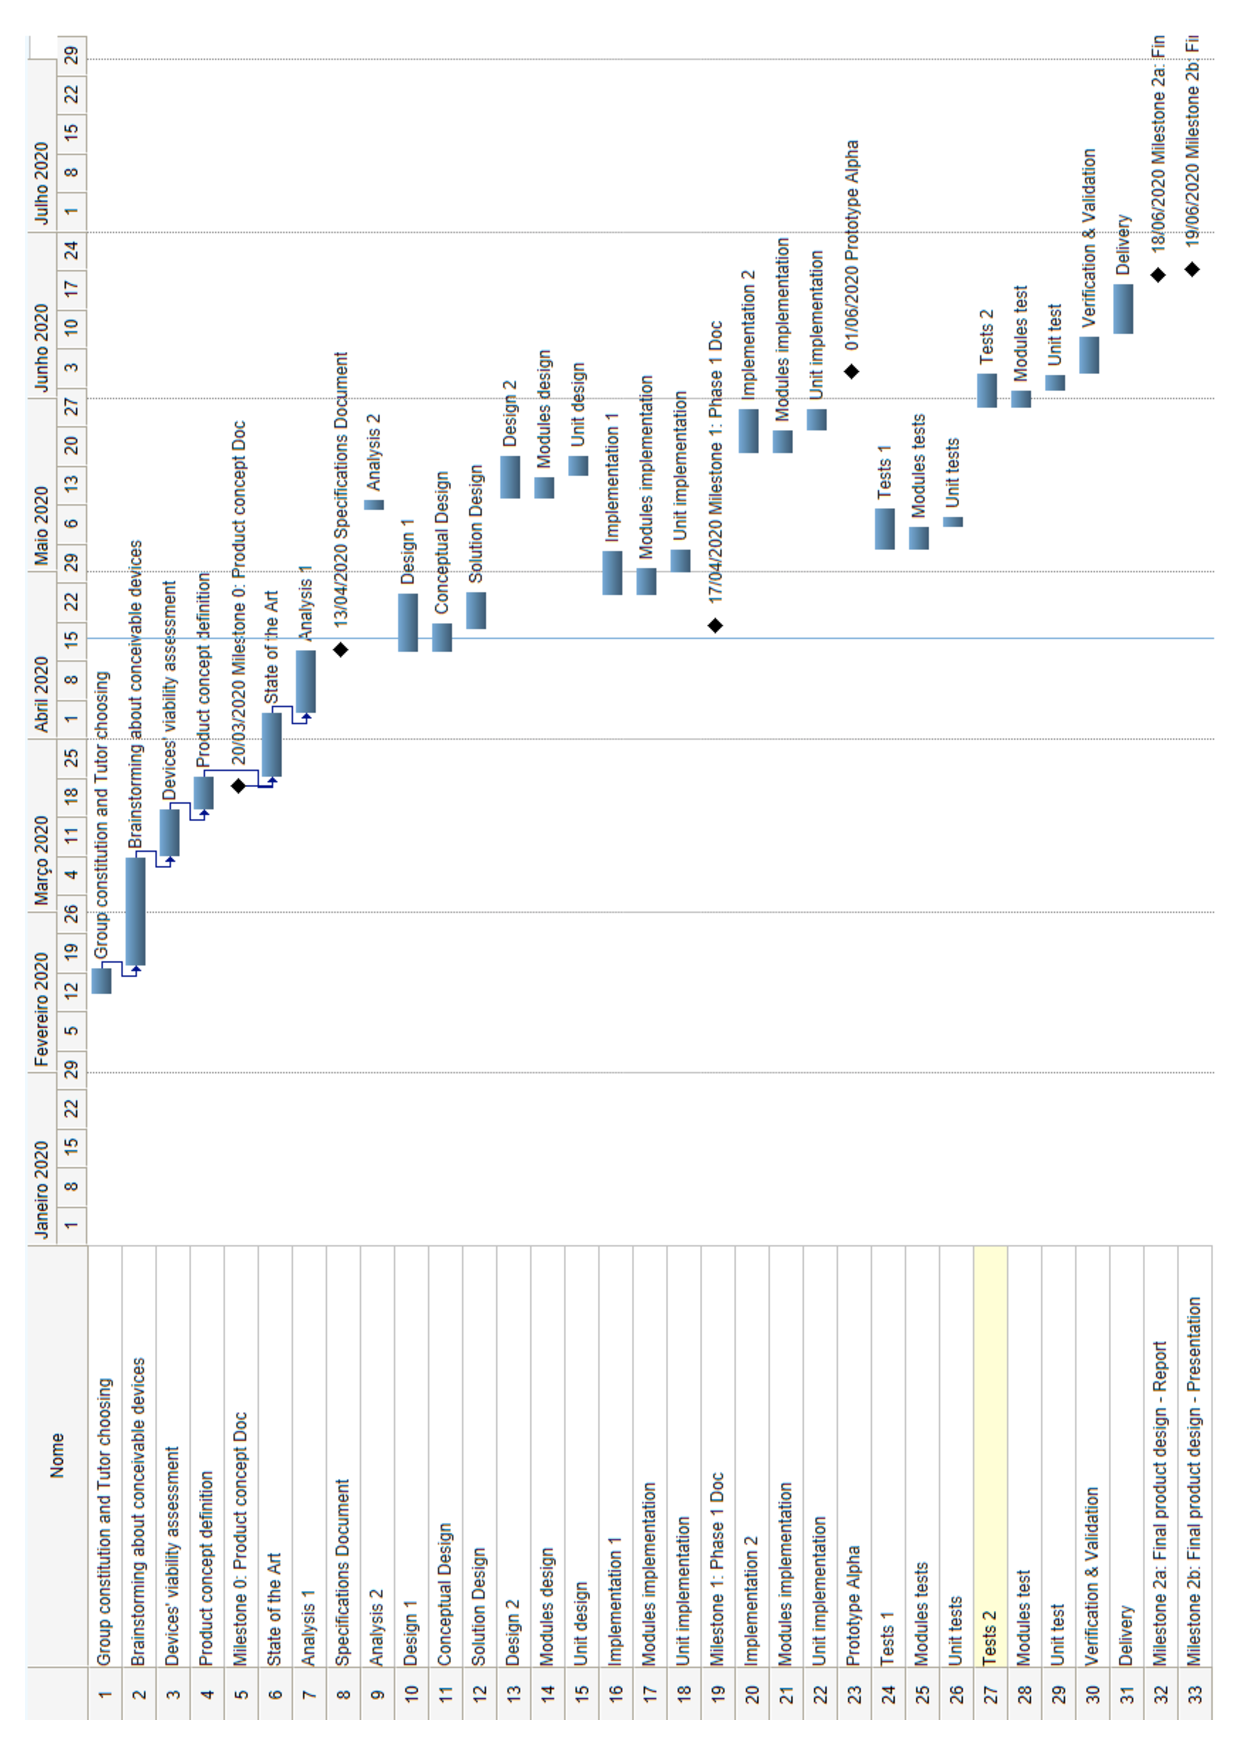
\includepdf[pages=-]{sec/pdf/gantt-diag-orig.pdf}
\begin{sidewaysfigure}[!htbp]
  \centering
  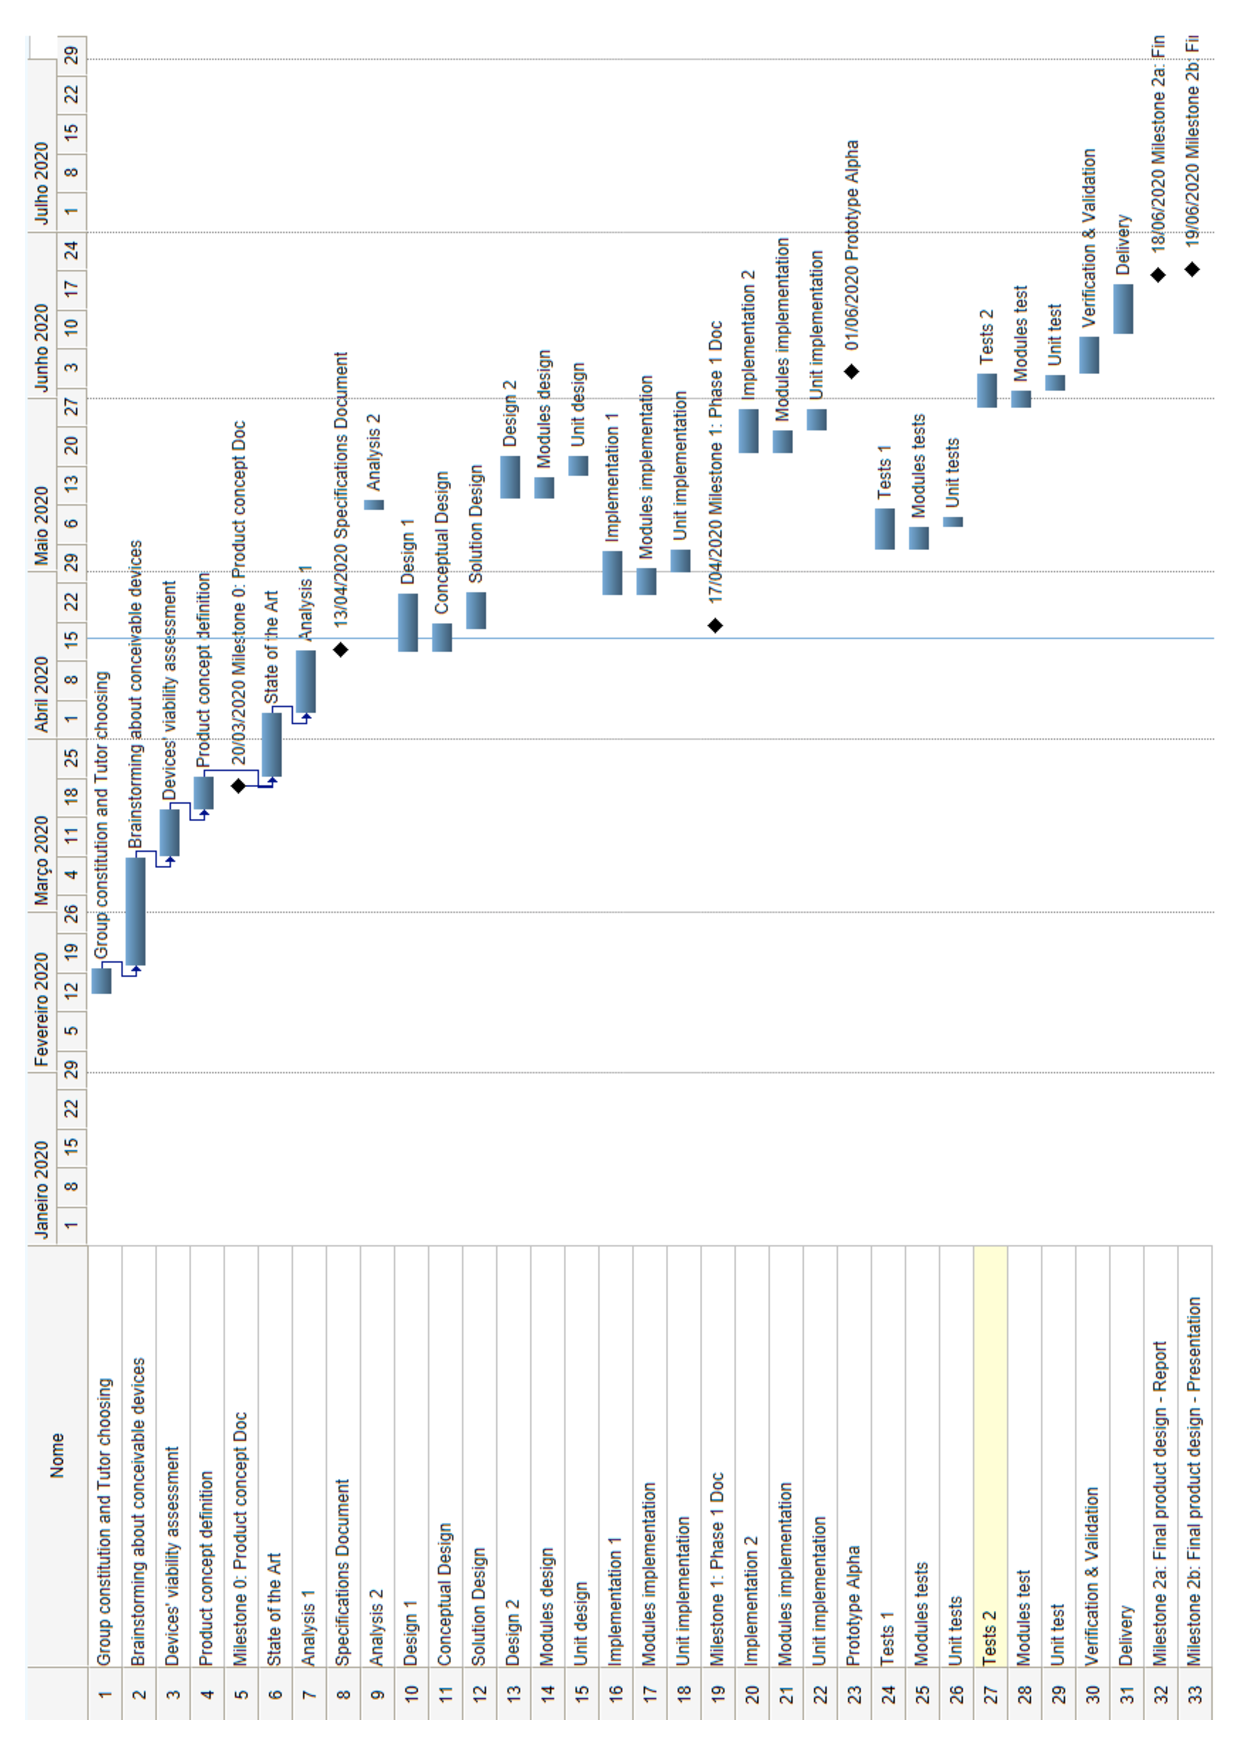
\includegraphics[page=1,width=1.0\textwidth]{sec/pdf/gantt-diag-orig.pdf} 
  \caption{Project planning --- Gantt diagram}%
  \label{fig:gantt-diag-orig}
\end{sidewaysfigure}
% 
%%% Local Variables:
%%% mode: latex
%%% TeX-master: "../Phase1"
%%% End:
